\documentclass[9pt,dvipsnames]{beamer}
\usepackage[T1]{fontenc}
\usepackage{libertinus}
\usepackage{amsmath}
\usepackage[most]{tcolorbox}

\usepackage{hyperref}

\usepackage{xcolor}  
\newcommand{\cb}[1]{{\color{CadetBlue}#1}}


\usetheme{Berkeley}
% \setbeamertemplate{footline}[frame number]
\setbeamertemplate{navigation symbols}{}


\title{CSE574 Introduction to Machine Learning}
\subtitle{Continual Learning}
\author{Jue Guo}
\institute{University at Buffalo}
\date{\today}

\begin{document}
\begin{frame}
    \titlepage
\end{frame}

\begin{frame}
    \frametitle{Outline}
    \tableofcontents
\end{frame}

\section{Abstract}
\begin{frame}{Abstract}
    To cope with real-world dynamics, an intelligent agent needs to incrementally acquire, update, accumulate, and exploit knowledge throughout its lifetime.
    \begin{itemize}
        \item \textbf{continual learning}, a fundation for AI systems to develop themselves adaptively. In a general sense, continual learning is explicitly limited by \textbf{catastrophic forgetting}, where learning a new task usually results in a dramatic performance degradation of the old tasks.
    \end{itemize}
\end{frame}

\section{Introduction}
\begin{frame}{Introduction}
    Learning is the basis for intelligent systems to accommodate environments. In response to external changes, evolution has empowered human and other organisms with strong adaptability to continually acquire, update, accumulate and exploit knowledge. Naturally we expect artifical intelligence (AI) systems to adapt in a similar way.
    \begin{itemize}
        \item This motivates the study of \textbf{continual learning}, where a typical setting is to learn a sequence of contents one by one and behave as if they were observed simultaneously. Such contents could be new skills, new examples of old skills, different environments, different contexts, etc., with particular realistic challenges incorporated.
        \item As the contents are provided incrementally over a lifetime, continual learnming is also referred to as \textbf{incremental learning} or \textbf{lifelong learning} in much of the literature, without a strict distinction.
    \end{itemize}
\end{frame}

\begin{frame}
    Unlike conventional machine learning models built on the premise of capturing a static data distribution, continual learning is characterized by learning from dynamic data distributions. A major challenge is known as \textbf{catastrophic forgetting}, where adaptation to a new distribution generally results in a largely reduced ability to capture old ones.
    \begin{itemize}
        \item This dilemma is a facet of the trade-off between \textbf{learning plasticity} and \textbf{memory stability}: an excess of the former interferes with the latter, and vice versa. A desirable solution for continual learning should obtain strong \textbf{generalizability} to accommodate distribution differences within and between tasks.
        \item A naive baseline, retraining all old training samples makes it easy to address the above challenges, but creates huge computational and storage overheads (as well as potential privacy issues).
    \end{itemize}
    In fact, continual learning is primarily intended to ensure the \textbf{resource efficiency} of model updates, perferably close to learning only new samples.
\end{frame}

\begin{frame}
    Numerous efforts have been devoted to addressing the above challenges, which can be conceptually seperated into five groups:
    \begin{enumerate}
        \item regularization-based approach
        \item replay-based approach
        \item optimization-based approach
        \item representation-based approach
        \item architecture-based approach
    \end{enumerate}
    These methods are \textit{closely connected}, e.g., regularization and replay ultimately act to rectify the gradient directions in optimization, and \textit{highly synergistic}, e.g., the efficacy of replay can be facilitated by distilling knowledge from the old model.
\end{frame}
\begin{frame}
    \begin{figure}[ht]
        \centering
        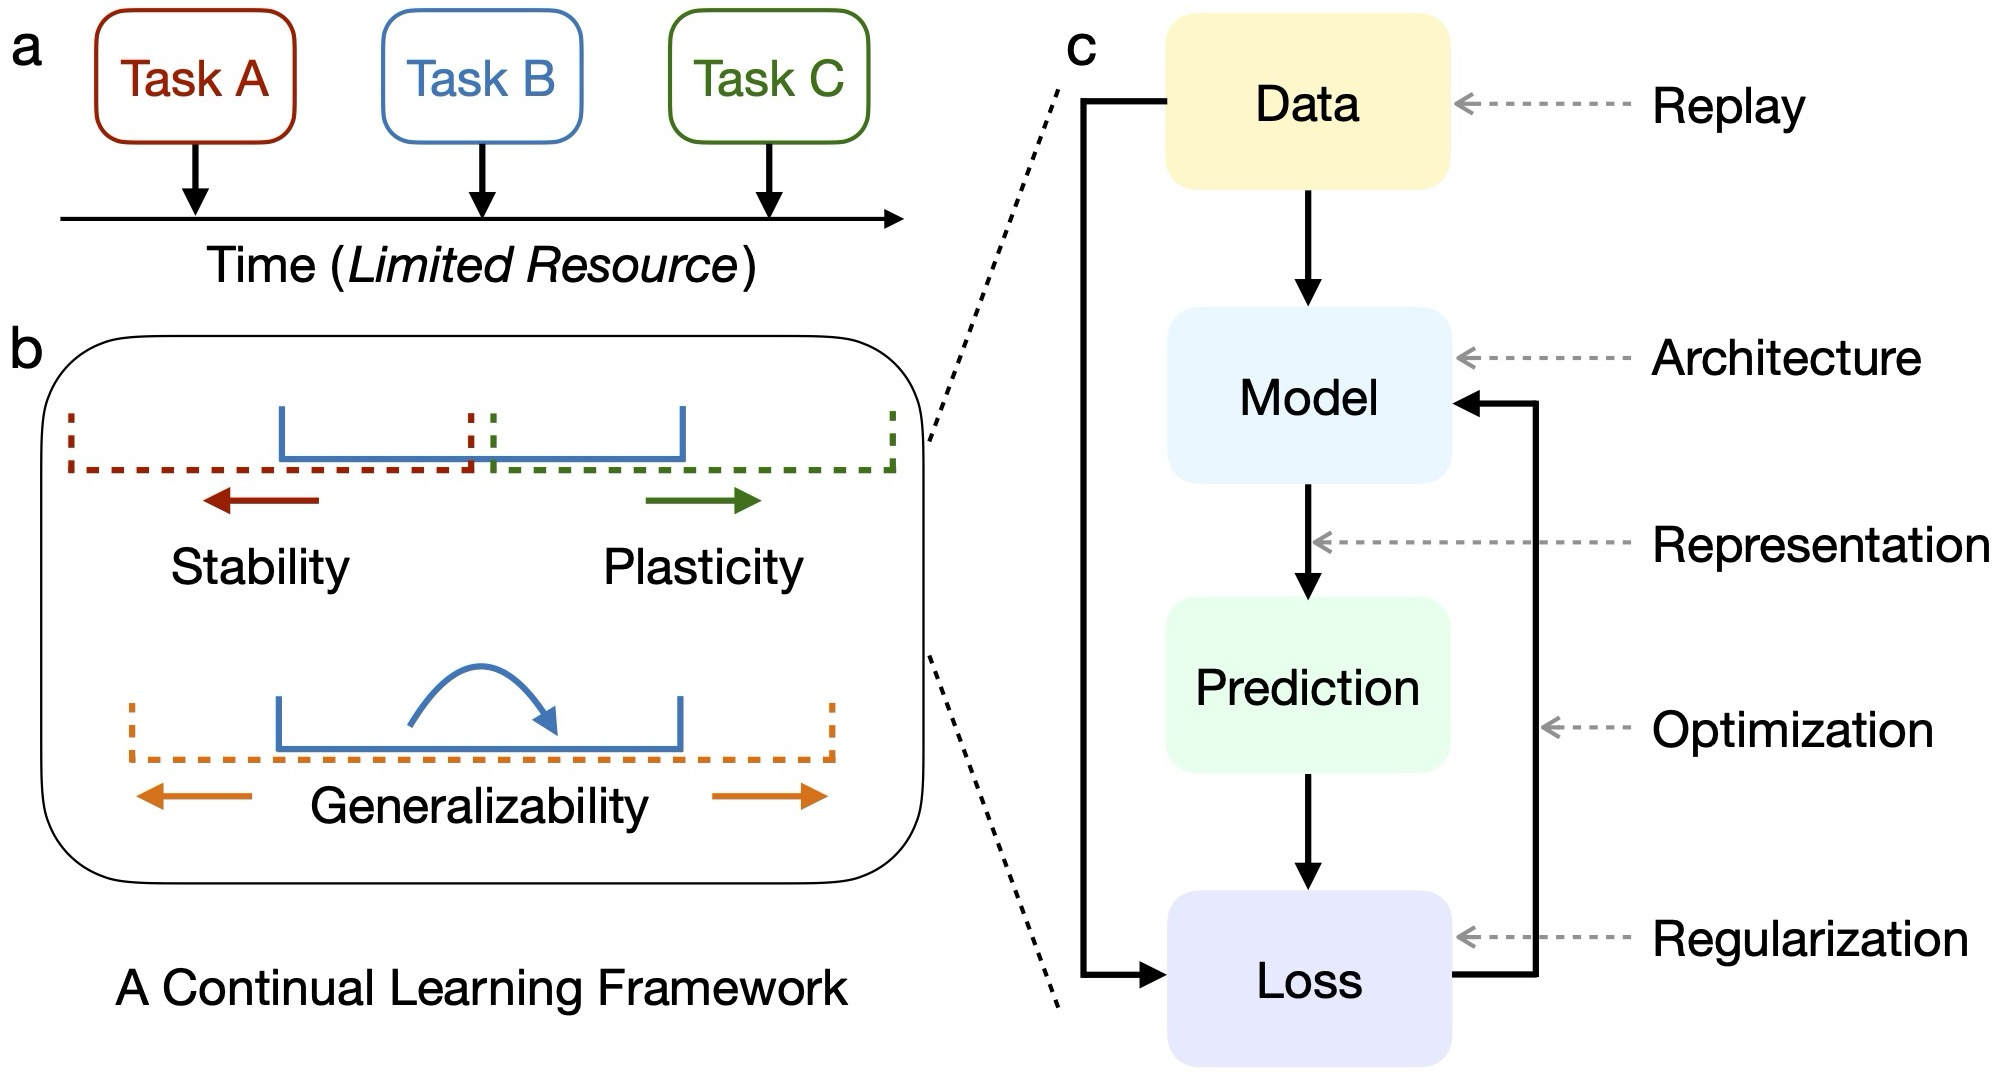
\includegraphics[width=0.5\linewidth]{imgs/cl_1.png}
        \caption{A conceptual framework of continual learning. \textbf{a}, Continual learning requires adapting to incremental tasks with dynamic data distributions. \textbf{b}, A desirable solution should ensure a proper balance between stability (red arrow) and plasticity (green arrow), as well as an adequate generalizability to intra-task (blue arrow) and inter-task (orange arrow) distribution differences. \textbf{c}, Representative strategies have targeted various aspects of machine learning.}
    \end{figure}
\end{frame}



\end{document}